\documentclass[11pt]{article}
\usepackage{a4wide}
%\raggedright
%\usepackage{driverbook}
\usepackage{latexsym}           % math symbols that were omitted in latex2e
\usepackage{amsbsy}             % bold greek defs
\usepackage{amsmath,graphicx}
\usepackage{bbm}
\usepackage{mathrsfs}
\usepackage{stmaryrd}
\usepackage{graphics}
\usepackage{acronym}
\usepackage{longtable}
\usepackage{mathtools}
\usepackage{times}
\usepackage{setspace}
\usepackage{cite}
\usepackage{array}
\usepackage{subfigure}
\usepackage{amsmath,amsthm}
\usepackage{amssymb}
\usepackage{wasysym,url}
\usepackage{fixltx2e,amsmath}
\usepackage{setspace,float}
\usepackage{color}
\usepackage{cases,bm}
\usepackage{mathrsfs}
\usepackage{enumitem}
\usepackage{hyperref}
\usepackage{mathtools,cuted}
\usepackage[linesnumbered,ruled,vlined]{algorithm2e}
\usepackage{epsfig}
\usepackage{color}
\DontPrintSemicolon

\usepackage{geometry}
 \geometry{
 a4paper,
 total={170mm,257mm},
 left=20mm,
 top=30mm,
 bottom=30mm,
 }
 
 
\usepackage{listings}
\usepackage{xcolor}

\definecolor{codegreen}{rgb}{0,0.6,0}
\definecolor{codegray}{rgb}{0.5,0.5,0.5}
\definecolor{codepurple}{rgb}{0.58,0,0.82}
\definecolor{backcolour}{rgb}{0.95,0.95,0.92}

\lstdefinestyle{mystyle}{
    backgroundcolor=\color{backcolour},   
    commentstyle=\color{codegreen},
    keywordstyle=\color{magenta},
    numberstyle=\tiny\color{codegray},
    stringstyle=\color{codepurple},
    basicstyle=\ttfamily\footnotesize,
    breakatwhitespace=false,         
    breaklines=true,                 
    captionpos=b,                    
    keepspaces=true,                 
    numbers=left,                    
    numbersep=5pt,                  
    showspaces=false,                
    showstringspaces=false,
    showtabs=false,                  
    tabsize=2
}

\lstset{style=mystyle}

\newcommand{\by}{\mathbf{y}}
\newcommand{\br}{\mathbf{r}}
\newcommand{\ba}{\mathbf{a}}
\newcommand{\bh}{\mathbf{h}}
\newcommand{\bx}{\mathbf{x}}
\newcommand{\be}{\mathbf{e}}
\newcommand{\bw}{\mathbf{w}}
\newcommand{\bR}{\mathbf{R}}
\newcommand{\bI}{\mathbf{I}}
\newcommand{\bA}{\mathbf{A}}
\newcommand{\bH}{\mathbf{H}}
\newcommand{\bQ}{\mathbf{Q}}
\newcommand{\bG}{\mathbf{G}}
\newcommand{\bC}{\mathbf{C}}
\newcommand{\rr}{\mathbb{R}}
\newcommand{\zz}{\mathbb{Z}}
\newcommand{\nn}{\mathbb{N}}
\newcommand{\cc}{\mathbb{C}}
\newcommand{\Ex}{\mathbb{E}}
\newcommand{\TT}{\mathsf{T}}
\newcommand{\HH}{\mathsf{H}}
\newcommand{\dd}{\mathrm{d}}
\newcommand{\jj}{\mathrm{j}}

\newcommand{\zerovec}{\boldsymbol{0}}
\newcommand{\bSigma}{\boldsymbol{\Sigma}}
\newcommand{\btheta}{\boldsymbol{\theta}}
\newcommand{\bgamma}{\boldsymbol{\gamma}}

\begin{document}
\thispagestyle{empty}

{\small
\begin{flushleft}
   Name: Abijith J. Kamath\\
   Student Id: 17788
\end{flushleft}
}
\vspace{2ex}
\begin{center}
    {\Large\bf E1 244: Detection and Estimation}\\
    February-May 2021

\vspace{5mm}
{\bf Solution -- Homework 2}
\end{center}
\vspace{5mm}

\section*{Analysis and Algorithms for Faulty Sensor Interpolation}

% -----------------------------------------------------------------------------------------------------------------------
% -----------------------------------------------------------------------------------------------------------------------

\subsection*{Part A: Derivation and Modelling}
\label{subsec:partA}
Consider the auto-regressive signal of order $1$ modelled using the parameter $\alpha \in \rr$ as: $x(n) = \alpha x(n-1) + w(n)$ where $w(n)$ is additive white Gaussian noise with variance $\sigma_{w}^{2}$. The measurements of the signal $x$ is incomplete with one sample missing at index $n_{0}$. The $N-1$ length measurement vector can be given as $\bx = [ x(0) \; x(1) \; \cdots \; x(n_{0}-1) \; x(n_{0}+1) \; \cdots \; x(N-1) ]^{\TT}$. The interpolation problem is to estimate the sample $x(n_{0})$ given complete or partial information $\bx$.

Consider the auto-regressive sequence of order $1$, modelled as
\begin{equation}
	x(n) = \alpha x(n-1) + w(n),
\label{eq:signalModel}
\end{equation}
where $w(n) \overset{\text{iid}}{\sim} \mathcal{N}(0, \sigma_{w}^{2})$. The autocorrelation sequence $r_{k} = \Ex[x(n) x(n-k)]$ can be computed as:
\begin{equation}
\begin{split}
	r_{k} &= \Ex[x(n) x(n-k)] \\
	&= \Ex \left[ (\alpha x(n-1) + w(n)) x(n-k) \right] \\
	&= \alpha \Ex \left[ x(n-1) x(n-k) \right] + \Ex \left[ w(n) x(n-k) \right] \\
	& \overset{(a)}{=} \alpha r_{k-1},
\end{split}
\end{equation}
where $(a)$ follows from assuming the noise and the signal are independent. The autocorrelation sequence has a recursive form, with
\begin{equation}
\begin{split}
	r_{0} &= \Ex \left[ (\alpha x(n-1) + w(n)) (\alpha x(n-1) + w(n)) \right], \\
	&= \Ex \left[ \alpha^{2} x(n-1) x(n-1) + 2\alpha x(n-1) w(n) + w(n) w(n) \right], \\
	&= \alpha^{2} r_{0} + \sigma_{w}^{2}, \\
	\implies r_{0} &= \frac{\sigma_{w}^{2}}{1-\alpha^{2}}.
\end{split}
\end{equation}

% -----------------------------------------------------------------------------------------------------------------------

\subsubsection*{Wiener Interpolator}
\label{subsubsec:wiener}

The full Wiener interpolator is a linear estimator that minimises the Bayesian mean-squared error (BMSE) using all the sample points in $\bx$. The Wiener interpolator is of the form $\hat{x}_{WF}(n_{0}) = \sum_{i=0, i\neq n_{0}}^{N-1} a_{i} x(i) = \ba_{WF}^\TT \bx$, where the weights of the linear interpolator are in the vector $\ba = [a_{0} \; a_{1} \; \cdots \; a_{n_{0}-1} \; a_{n_{0}+1} \; \cdots \; a_{N-1}]^{\TT}$. The BMSE of some estimator $\hat{x}(n_{0})$ as a function of the weight vector $\ba$:
\begin{equation}
\begin{split}
	bmse(\hat{x}(n_{0})) &= \Ex \left[ \left( x(n_{0}) - \hat{x}(n_{0}) \right)^{2} \right], \\
	&= \Ex \left[ x(n_{0})x(n_{0}) - 2x(n_{0}) \ba^{\TT}\bx + \ba^{\TT} \bx \bx^{\TT} \ba \right].
\end{split}
\label{eq:bmse}
\end{equation}
The Wiener interpolator is the minimiser of BMSE with respect to the weights $\ba$. The Wiener interpolator has weights that satisfy the equation:
\begin{equation}
	\frac{\partial}{\partial \ba} bmse(\hat{x}_{WF}(n_{0})) = \Ex \left[ -2 x(n_{0})\bx + 2\bx\bx^{\TT} \ba_{WF} \right] = \zerovec,
\end{equation}
i.e., the weights satisfy the linear system of equations $\Ex [\bx\bx^{\TT}] \ba_{WF} = \Ex[x(n_{0}) \bx]$:
\begin{equation}
	\underbrace{\begin{bmatrix}
		r_{0} & r_{1} & \cdots & r_{n_{0}-1} & r_{n_{0}+1} & \cdots & r_{N-1} \\
		r_{1} & r_{0} & \cdots & \cdots & \cdots & \cdots & r_{N-2} \\
		\vdots & \vdots & \vdots & \vdots & \vdots & \vdots & \vdots \\
		r_{n_{0}-1} & \vdots & \vdots & \vdots & \vdots & \vdots & \vdots \\
		r_{n_{0}+1} & \vdots & \vdots & \vdots & \vdots & \vdots & \vdots \\
		\vdots & \vdots & \vdots & \vdots & \vdots & \vdots & \vdots \\
		r_{N-1} & r_{N-2} & \cdots & \cdots & \cdots & \cdots & r_{0}
	\end{bmatrix}}_{\mathbf{R}_{WF}} \ba_{WF} = 
	\underbrace{\begin{bmatrix}
		r_{n_{0}} \\ r_{n_{0}-1} \\ \vdots \\ r_{1} \\ r_{1} \\ \vdots \\ r_{N-n_{0}-1}
	\end{bmatrix}}_{\mathbf{r}_{WF}}.
\label{eq:WFlinearSystem}
\end{equation}
Therefore, the Wiener interpolator has weights $\ba_{WF} = \bR_{WF}^{-1} \br_{WF}$, and hence $\hat{x}_{WF}(n_{0}) = {\ba_{WF}}^{\TT}\bx$. Using this in (\ref{eq:WFbmse}),
\begin{equation}
\begin{split}
	bmse(\hat{x}_{WF}(n_{0})) &= \Ex \left[ x(n_{0})x(n_{0}) - 2x(n_{0}) \bx^{\TT} \bR_{WF}^{-1} \br_{WF} + \br_{WF}^{\TT} \bR_{WF}^{-T} \bx \bx^{\TT} \bR_{WF}^{-1} \br_{WF} \right], \\
	&= r_{0} - 2 \br_{WF}^{\TT} \bR_{WF}^{-1} \br_{WF} + \br_{WF}^{\TT} \bR_{WF}^{-1} \br_{WF}, \\
	&= r_{0} - \br_{WF}^{\TT} \bR_{WF}^{-1} \br_{WF}.
\end{split}
\label{eq:WFbmse}
\end{equation}

% -----------------------------------------------------------------------------------------------------------------------

\subsubsection*{Two-Point-Average Interpolator}
\label{subsubsec:avginterp}

The two-point average (TPA) interpolator is a linear estimator that minimises the BMSE using the adjacent samples to the missing sample. The TPA interpolator has the form $\hat{x}_{TPA}(n_{0}) = a_{1}x(n_{0}-1) + a_{2}x(n_{0}+1)$, where $\ba_{TPA} = [a_{1} \; a_{2}]^{\TT}$ are the parameters of the estimator. An estimator with this structure is similar to the Wiener interpolator where the coefficients other than that of $x(n_{0}-1)$ and $x(n_{0}+1)$ are set to zero. The corresponding solution is obtained from (\ref{eq:WFlinearSystem}) by taking the $2\times 2$ block:
\begin{equation}
	\underbrace{\begin{bmatrix}
		r_{0} & r_{2} \\
		r_{2} & r_{0}
	\end{bmatrix}}_{\bR_{TPA}} \ba_{TPA} = 
	\underbrace{\begin{bmatrix}
		r_{1} \\ r_{1}
	\end{bmatrix}}_{\br_{TPA}}.
\end{equation}
Therefore, the two-point average interpolator has weights $\ba_{TPA} = \bR_{TPA}^{-1}\br_{TPA}$, and hence $\hat{x}_{TPA}(n_{0}) = \ba_{TPA}^{\TT} [x(n_{0}-1) \; x(n_{0}+1)]^{\TT}$. The solution here can be obtained in closed form with $\displaystyle a_{1} = a_{2} = \frac{\alpha}{1+\alpha^{2}}$. Similar to the calculation in (\ref{eq:WFbmse}), the BMSE for TPA interpolator is:
\begin{equation}
	bmse(\hat{x}_{TPA}(n_{0})) = r_{0} - \br_{TPA}^{\TT} \bR_{TPA}^{-1} \br_{TPA}.
\label{eq:TPAbmse}
\end{equation}


% -----------------------------------------------------------------------------------------------------------------------

\subsubsection*{Causal Wiener Interpolator}
\label{subsubsec:causalwiener}

The causal Wiener (CWF) interpolator is a linear estimator that minimises the BMSE using only the previous samples to the missing samples. The CWF interpolator has the form $\hat{x}_{CWF}(n_{0}) = \sum_{i=0}^{n_{0}-1} a_{i} x(i)$, where $\ba_{CWF} = [a_{0} \; a_{1} \; \cdots \; a_{n_{0}-1}]^{\TT}$ are the parameters of the estimator. This is similar to the structure in the Wiener filter with the coefficients of the positive delays set to zero. The corresponding solution is obtained from (\ref{eq:WFlinearSystem}) by taking the top right $n_{0} \times n_{0}$ block:
\begin{equation}
	\underbrace{\begin{bmatrix}
		r_{0} & r_{1} & \cdots & r_{n_{0}-1} \\
		r_{1} & r_{0} & \cdots & r_{n_{0}-2} \\
		\vdots & \vdots & \vdots & \vdots \\
		r_{n_{0}-1} & \cdots & \cdots & r_{0} \\
	\end{bmatrix}}_{\mathbf{R}_{CWF}} \ba_{CWF} = 
	\underbrace{\begin{bmatrix}
		r_{n_{0}} \\ r_{n_{0}-1} \\ \vdots \\ r_{1}
	\end{bmatrix}}_{\mathbf{r}_{WF}}.
\label{eq:WFlinearSystem}
\end{equation}
Therefore, the causal Wiener interpolator has weights $\ba_{CWF} = \bR_{CWF}^{-1}\br_{CWF}$, and hence $\hat{x}_{CWF}(n_{0}) = \ba_{CWF}^{\TT} [x(0) \; \cdots \; x(n_{0}-1)]^{\TT}$. Similar to the calculation in (\ref{eq:WFbmse}), the BMSE for TPA interpolator is:
\begin{equation}
	bmse(\hat{x}_{CWF}(n_{0})) = r_{0} - \br_{CWF}^{\TT} \bR_{CWF}^{-1} \br_{CWF}.
\label{eq:CWFbmse}
\end{equation}

% -----------------------------------------------------------------------------------------------------------------------

\subsubsection*{Kalman Filter}
\label{subsubsec:kalman}

Suppose the measurements of the signal be noisy, i.e., $y(n) = x(n) + v(n)$, where $v(n) \overset{\text{iid}}{\sim} \mathcal{N}(0, \sigma_{v}^{2})$. The observation matrix is identity. The state evolution is given by the auto-regressive process with order $1$ as in (\ref{eq:signalModel}), and the state-transition matrix is the scalar $\alpha$. With some initialisation for the signal $\hat{x}(0 | 0)$ and variance of the error $P(0|0)$, the Kalman filter predictions are given as:
\begin{equation}
\begin{split}
	\hat{x}(n|n-1) &= \alpha \hat{x}(n-1 | n-1), \\
	P(n | n-1) &= \alpha^{2}P(n-1 | n-1) + \sigma_{w}^{2}.
\end{split}
\end{equation}
The Kalman gain is defined as $K(n) = P(n | n-1) \left( \sigma_{v}^{2} + P(n | n-1) \right)^{-1}$. The update on the signal and the variance of the error are given by:
\begin{equation}
\begin{split}
	\hat{x}(n|n) &= \hat{x}(n | n-1) + K(n) \left( y(n) + \hat{x}(n | n-1) \right), \\
	P(n | n) &= (1 - K(n)) P(n | n-1).
\end{split}
\end{equation}

% -----------------------------------------------------------------------------------------------------------------------
% -----------------------------------------------------------------------------------------------------------------------

\subsection*{Part B: Implementation}
\label{subsec:partB}

Figure \ref{fig:wiener} shows Monte-Carlo simulation of interpolation using Wiener interpolation methods. The auto-regressive signal of order $1$ with varying $\alpha$ from $0.1$ to $0.9$ are taken with noise variance fixed at $\sigma_{w}^{2} = 0.36$. The same signal is subject to interpolation at index $40$ using three methods based on the Wiener filter idea. The errors upon averaging over $1000$ realisations are shown in Figure \ref{fig:wiener}.

\begin{figure}[t]
\centering
\subfigure[]{\label{fig:a}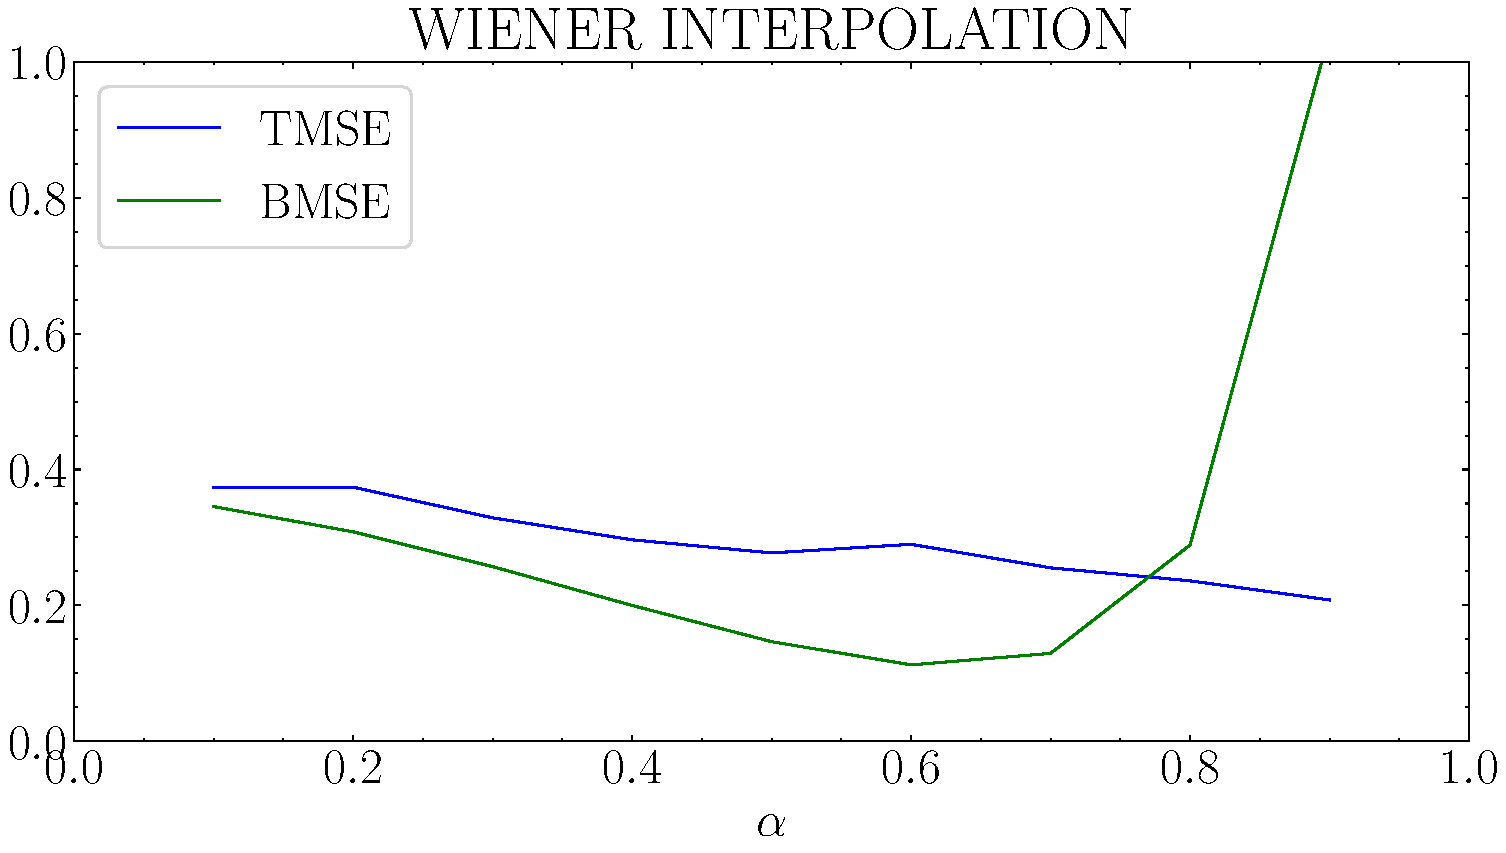
\includegraphics[width=3in]{../results/wiener1.pdf}}
\subfigure[]{\label{fig:b}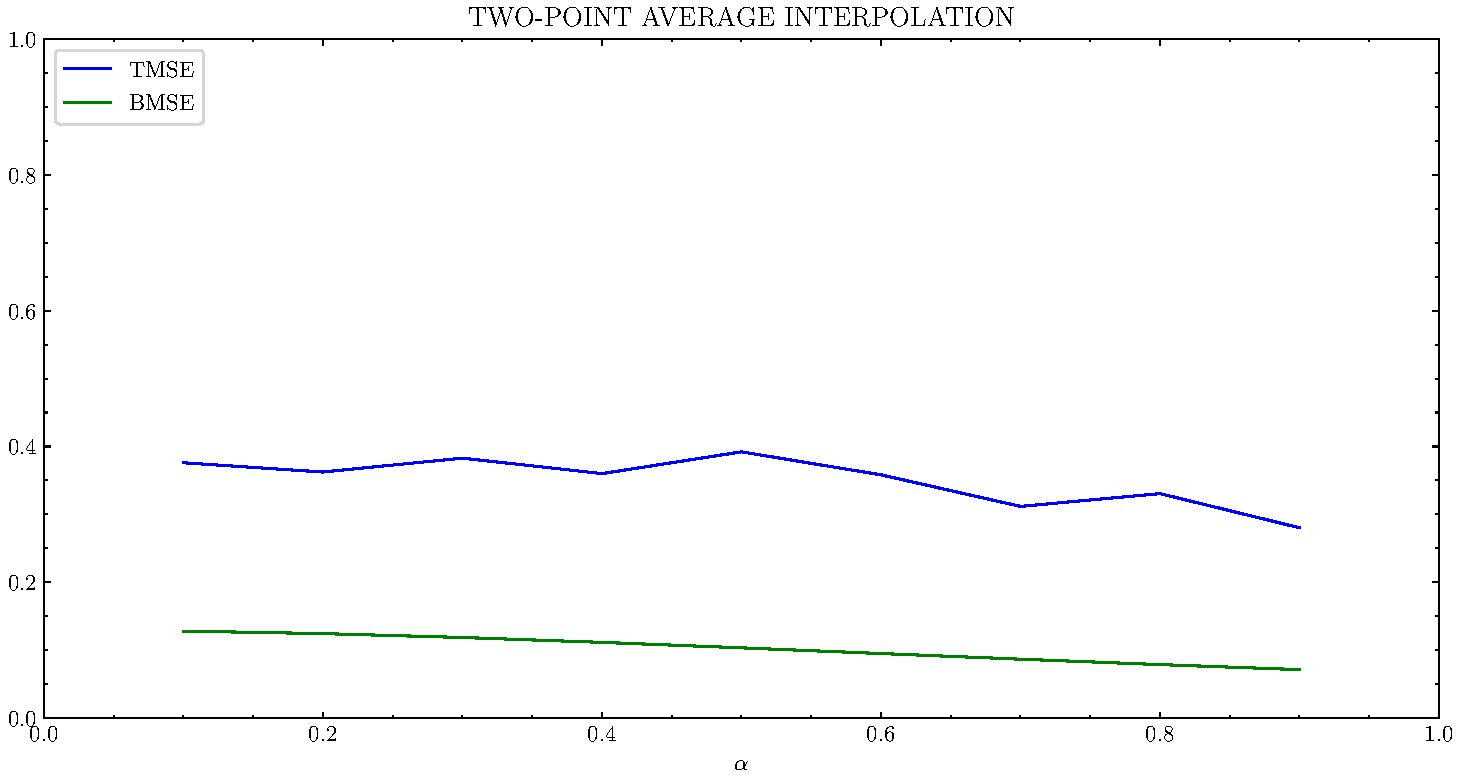
\includegraphics[width=3in]{../results/wiener2.pdf}}
\subfigure[]{\label{fig:c}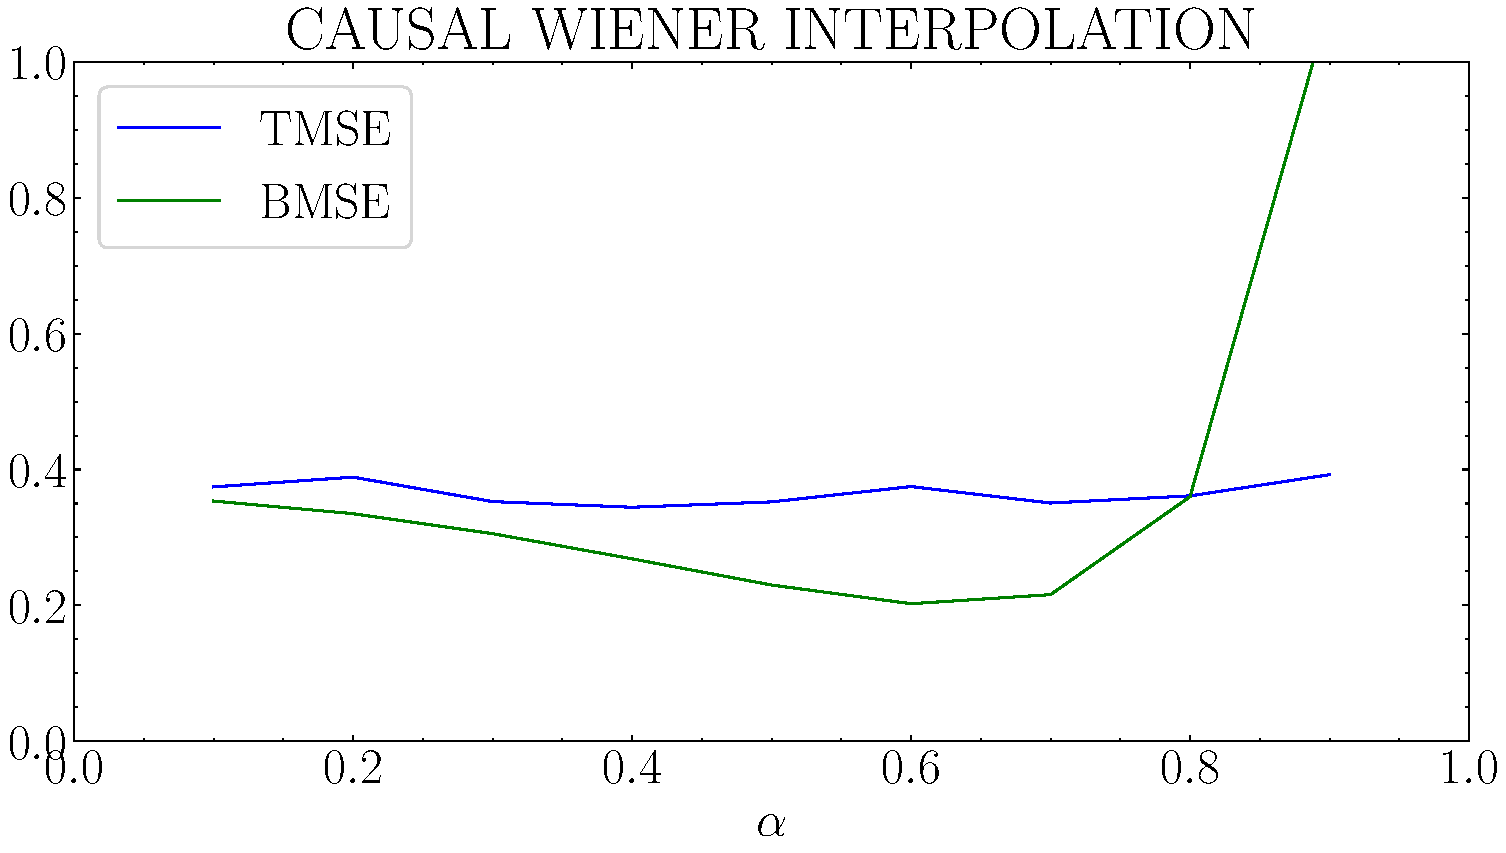
\includegraphics[width=3in]{../results/wiener3.pdf}}
\caption{Monte-Carlo analysis of interpolation using Wiener interpolation methods.}
\label{fig:wiener}
\end{figure}

% -----------------------------------------------------------------------------------------------------------------------

\subsubsection*{Wiener Interpolator}
\label{subsubsec:wienerimplementation}

Figure \ref{fig:wiener}(a) shows the Monte-Carlo simulation using complete Wiener filter. The BMSE decreases with $\alpha$ increasing up to $0.6$, and then increases. The theoretical mean-squared error (TMSE) shows a decreasing trend with increasing $\alpha$. It can be seen that the BMSE can be lower than the TMSE, which is indicative of Bayesian methods that introduce bias to reduce the error. As $\alpha$ increases, the signal is approximately a constant buried in noise, where the estimation becomes difficult.

% -----------------------------------------------------------------------------------------------------------------------

\subsubsection*{Two-Point-Average Interpolator}
\label{subsubsec:avgimplementation}

Figure \ref{fig:wiener}(b) shows the Monte-Carlo simulation using two-point average interpolation. The BMSE and TMSE decrease with $\alpha$ and the BMSE is always lower than the TMSE. The two-point average interpolation only considers the relevant sample points and therefore is numerically more stable.

% -----------------------------------------------------------------------------------------------------------------------

\subsubsection*{Causal Wiener Interpolator}
\label{subsubsec:causalimplementation}

Figure \ref{fig:wiener}(c) shows the Monte-Carlo simulation using causal Wiener interpolation. The BMSE decreases with $\alpha$ increasing up to $0.6$, and then increases. The theoretical mean-squared error (TMSE) shows a decreasing trend with increasing $\alpha$. The errors are higher than the errors using the complete Wiener interpolation as shown in Figure \ref{fig:wiener}(a) as the complete Wiener interpolation uses more samples than the causal Wiener interpolation.

% -----------------------------------------------------------------------------------------------------------------------

\subsubsection*{Kalman Filter}
\label{subsubsec:kalmanimplementation}

Figure \ref{fig:kalman} shows the results of interpolation using Kalman filter. The auto-regressive signal of order $1$ with $\alpha = 0.8$ is taken with noise variance $\sigma_{w}^{2} = 0.36$. The signal is measured directly with Gaussian measurement noise of variance $\sigma_{w}^{2} = 1$. Figure \ref{fig:kalman}(a) shows the true signal and the estimated signal. It can be seen that the estimated signal follows the true signal with an approximately constant delay. This can be seen in \ref{fig:kalman}(b) with the errors saturating at constant values. The errors are high initially as the random initialisations maybe inaccurate, however, with future updates the errors settle.

\begin{figure}[t]
\centering
\subfigure[]{\label{fig:a}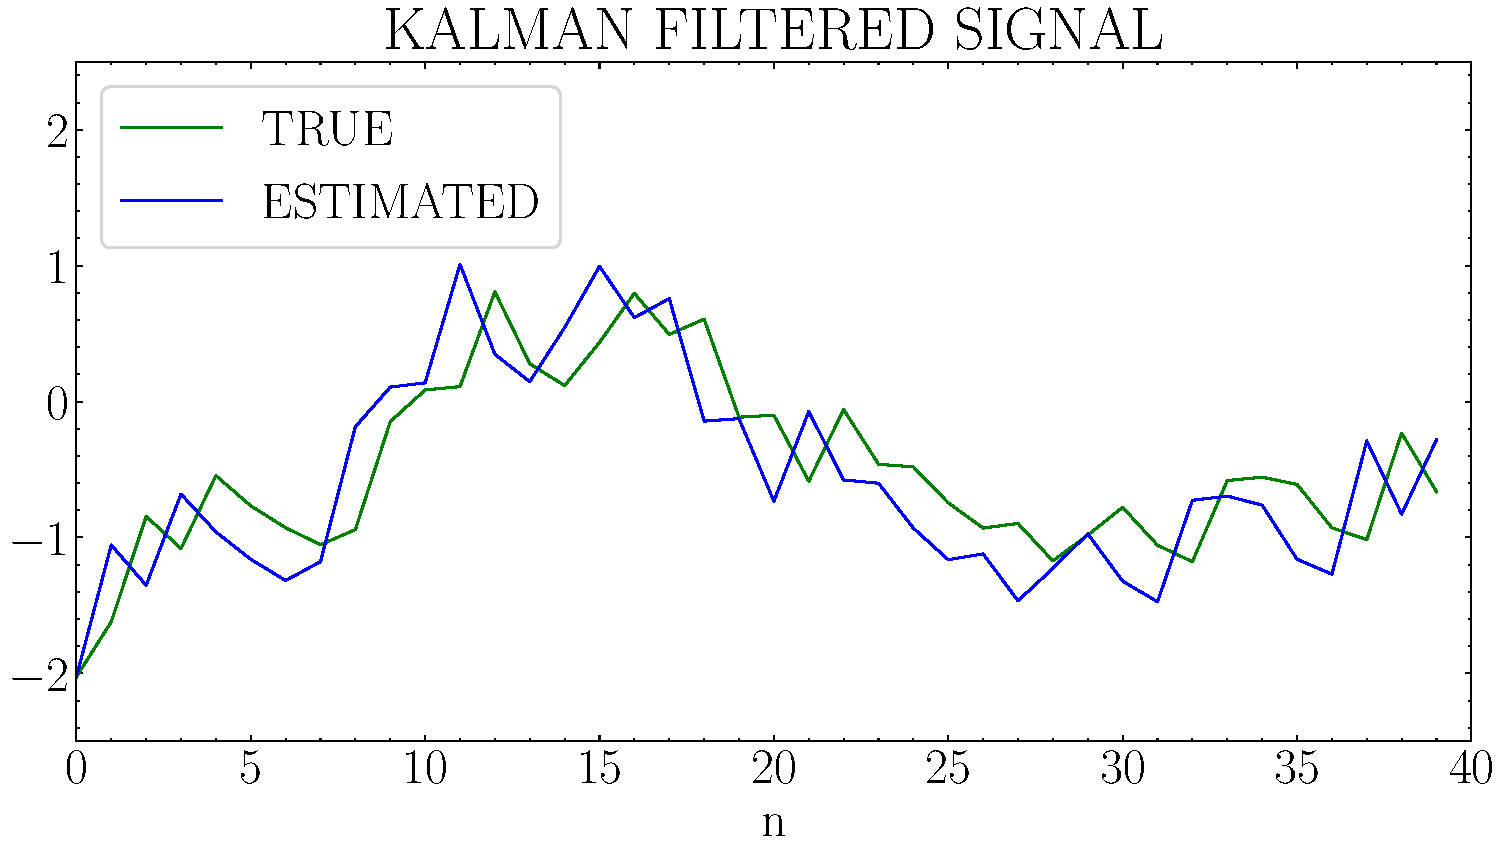
\includegraphics[width=3in]{../results/kalman1.pdf}}
\subfigure[]{\label{fig:b}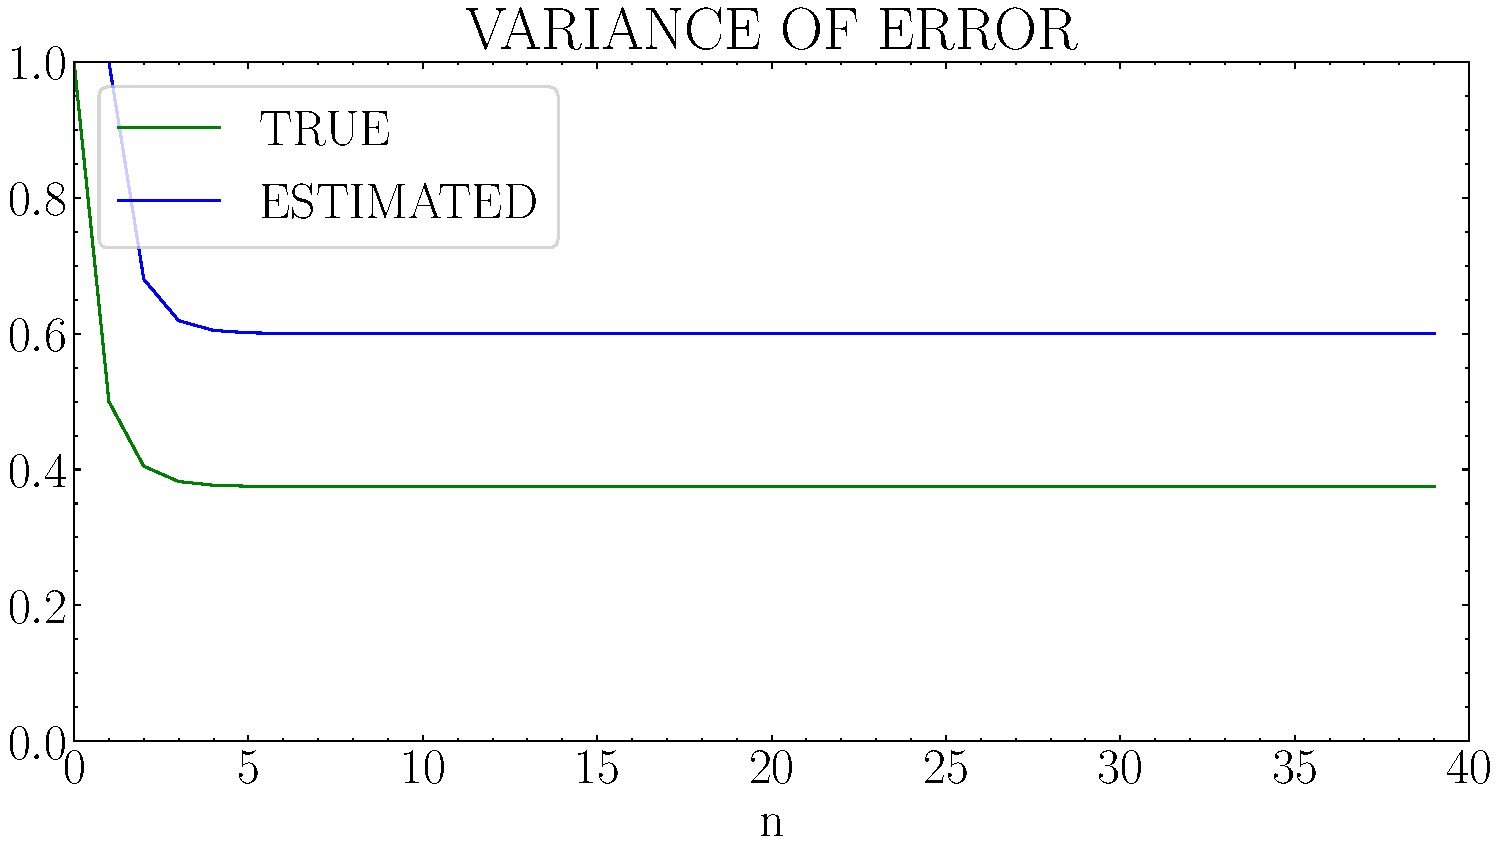
\includegraphics[width=3in]{../results/kalman2.pdf}}
\caption{Interpolation using Kalman filter.}
\label{fig:kalman}
\end{figure}

% -----------------------------------------------------------------------------------------------------------------------

\subsubsection*{Comparison: Causal Wiener Interpolation vs. Kalman Filter}
\label{subsubsec:comparison}


% -----------------------------------------------------------------------------------------------------------------------
% -----------------------------------------------------------------------------------------------------------------------

\appendix

\subsection*{Scripts}

% -----------------------------------------------------------------------------------------------------------------------

\subsubsection*{Implementation of Wiener Interpolator}


% -----------------------------------------------------------------------------------------------------------------------

\subsubsection*{Implementation of Two-Point-Average Interpolator}


% -----------------------------------------------------------------------------------------------------------------------

\subsubsection*{Implementation of Causal Wiener Interpolator}


% -----------------------------------------------------------------------------------------------------------------------

\subsubsection*{Implementation of Kalman Filter}


\end{document}
